\documentclass[a4paper,10pt]{article}
\usepackage[utf8]{inputenc}
\usepackage{graphicx}
\usepackage{pdflscape}
\usepackage{csquotes}
\usepackage{cite}
\usepackage[colorlinks=true,allcolors=black]{hyperref}
\title{Towards Best Practices for Chatbots}
\author{Maria Ferman}

\begin{document}

\maketitle
%chatbots to try: https://codurance.com/2017/02/08/the-4-key-elements-of-a-conversation/
% interface-platform
% Rapid prototyping and conversational flow https://www.behance.net/gallery/37453869/Designing-a-Chatbot-UX-Design-Process-Case-Study

%Chatbot definition (other)
%https://chatbotsmagazine.com/how-chatbots-can-help-your-users-without-you-there-e82e6814a903
%Chatbots provide a quicker response and better user experience by being “there.!!!

Users without any technological background require software that is accessible and customized to their needs. Fortunately, chatbots can help with both issues. Chatbots allow users to interact and communicate with software through their own words. Thus, software can become easier to understand and use. The efficiency of the chatbots can be augmented by considering the user preferences to allow software adapt to his or hers needs. According to Shevat,  ``Bots are a new user interface which let users interact with services and brands using their favorite messaging apps. Bots are a new way to expose software through a conversational interface"~\cite{Shevat2017}. 

In order to make the interaction between the user and the chatbot more efficient, designers require a comprehensive list of best practices about chatbot design. 
The design of a chatbot is more effective when designers use specific practices to avoid starting from scratch, as they give them a specific structure of how to design an efficient chatbot. 

\subsection*{Objective}

%To design and develop a chatbot in order to help novice users to create visualizations that allows them to analyse their data and discover deeper insights. The design of the chatbot will be carried out by developing a set of best practices that allow designers to efficiently create a text-based chatbot.  

To develop a set of best practices that allow designers to efficiently create and design a text-base chatbot. 

%Challenges:
%-to have a well design chatbot
%	+ one purpose oriented to the audience 
%	+...
%-As chatbots move into group chat settings, they’ll need to be designed to understand some of these contextual clues that form the basis for how people interact.
%(significant challenge for designers)
%-conversational flows are hard to design (not all the people know this)

%-Artificial intelligence isn’t just about smarts–it’s about social intelligence, -Xiaoice - https://www.fastcodesign.com/3064710/the-challenge-of-designing-a-chatbot-with-manners
%The chatbot’s sole purpose is to provide entertainment and companionship.!!!!

\subsection*{Motivation}

%To help designers to effectively create chatbots by having a complete and accurate set of best practices. This best practices will allow users to have a specific guide (steps) about the chatbot's creation. The best practices will describe the necessary elements that integrate chatbot.     

%How to create designers to have more effective visualizations X chatbot  
%to help visualization users novices from the designer point of view - best practices help them 

%Understanding data can be a difficult process for people without experience for creating visualizations. For example, project managers need to extract insights and discover patters in their data, and this may not be a straightforward process by using an excel table. Visualizations makes easy for novices to understand their data. However, creating visualization is also a complicated task for novice people. Chatbots can help in the visualization creation and data analysis process. By interacting with a chatbot, novices can get help or an additional support for the visualization creation and visual data exploration.

Creating a chatbot is not a straightforward task. Designers must keep in mind several elements in order to create it. They need to fully understand the task that they want to accomplish. In other words, what is the problem they want to solve, and think about the best solution. Many designers in chatbot creation agree that mapping a full conversation is one of the hardest elements to do~\cite{OreillyBots, ConversationHurtOrHelp?}. Designers need to fully understand the conversational script and flow that the chatbot needs to follow. 
%At the same time, the chatbot needs to be not only useful but also to have emotional and social intelligence in order to interact with users and help them to deal with the problem that they are sharing. 

Therefore, it is important for designers who want to create chatbots, to find a complete set of best practices to create and design a chatbot. There are several best practices and guidelines to create a chatbot~[\ref{FigureReferencetable}]. However, to the best of my knowledge they are not a complete set of best practices. This makes the chatbot creation process complicated and time consuming. These best practices will allow users to have specific steps about the chatbot's creation. The best practices will describe the necessary elements of a chatbot.     

%1.- Problema
%2.- Porque los gyidelines son necesarios
%3.- Trabajo previo, pero tal .. peor por esta razon ellos no solucionan el problema  

\section*{Project Description}

This project consists of three main phases. \textbf{The first phase} comprises the creation of a set of best practices to design chatbots effectively, based on well known online best practices. In order to develop a good set of best practices, it will be necessary to read blogs and best practices online (cf. Fig. \ref{FigureReferencetable}). Besides, it is also necessary to select and use the most popular chatbots. 
%See~(\ref{FigureReferencetable}).
\textbf{The second phase} is the mock-up of a visualization chatbot designed according to the best practices of the first phase. The visualization interface will be mimicked by using the \textit{Wizard of Oz} simulation technique. 
\begin{displayquote}
According to Hutchby~\cite{Hutchby2001} \textit{``Wizard of Oz} is a technique that involves humans masquerading as computer systems which are in the process of development, while the users recruited to test the ``system" are led to believe that it is actually a computer with which they are interacting.  The simulation is used as a test-bed in which ideas about how the system should operated, as well as how humans may interact with the system, can be explored by designers." 
\end{displayquote}

Finally, \textbf{the third phase} is the case study. This study will be carried out to evaluate the chatbot best practices. Therefore, if the chatbot fulfils the user requirements in the case study, this is a clear indication that the best practices are adequate for the creation of a chatbot.


% the chatbots' efficiency in interaction with the users in order to create effective visualizations.
 %PROJECT LIMITATIONS
 %The limitation is that it is subjective, it iwll take more time to fully validate it. 
 

%PARAGRAPH TO DESCRIBE THE TWO DIFFERENT PERSONAS. 
\subsection*{Project Personas}
The description of a persona, is used by designers to have an archetypal user of a system. Thus, the user-persona will illustrate the specific needs and goals that the system will satisfy~\cite{cooper2004inmates}.
This project has two personas that allow to understand the user type for the best practices and the visualisation chatbot.  

The first user-persona is defined as the type of person that will use the Chatbot's best practices (cf. Fig. \ref{FigurePatricia}). \textit{``Patricia"} is a developer who works in a startup company in Victoria, BC. She holds a Computer Science degree and has good programming skills. However, Patricia does not have experience designing chatbots. She lacks skills in and knowledge of software design. She has little time and lacks motivation to read blogs and best practices online. In addition, she finds the amount of chatbots blogs overwhelming. Therefore, her goal is to find a set of guidelines that help her to design a chatbot effectively. 

The second user-persona is the type of person that will use the visualization chatbot (cf. Fig. \ref{FigureLaura}). \textit{``Laura"} is a Visualization novice who works as a project manager in a mid-sized company in Victoria, BC. She has managed several projects successfully. However, she does not have any background creating visualizations. On a daily basis, she uses her computer, iPad, and mobile phone to work. She has problems in creating visualizations to explain her ideas and project results. She has little time to devote to the visualization creation process, and struggles in learning new technologies. Besides, she finds the amount of visualization tools overwhelming. Laura would like to find a good way, by using her mobile phone, to create an effective visualization. In addition, she would like to get help in the visualization creation and data analysis process.  


\begin{landscape}
\begin{figure}[p]
\thispagestyle{empty}
\vfill
    \makebox[\linewidth]{
        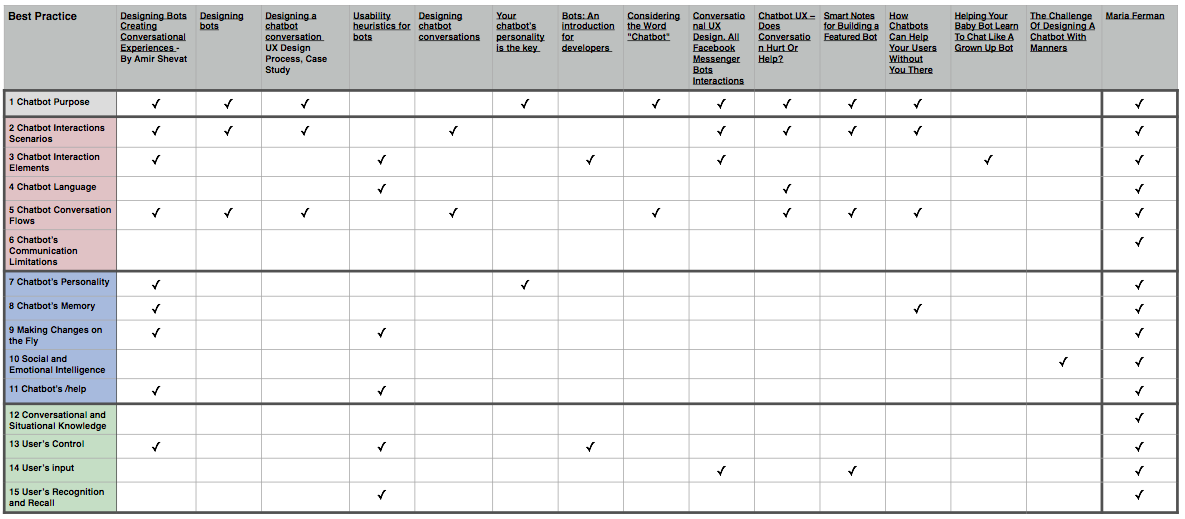
\includegraphics[width=1.4\linewidth]{/Users/MariaFerman/Desktop/ToRead(Project:Bots)/imgDesignfesst/ReferenceTable.png}}
    \caption{Best Practices' Reference}
\begin{center}    
    {\thepage}
\end{center}
    \label{FigureReferencetable}
\end{figure}
\end{landscape}

\begin{figure}
\centering
\includegraphics[scale=0.4]{/Users/MariaFerman/Desktop/ToRead(Project:Bots)/LaTexImages/BestPracticesPersona.png}
\caption{Characteristics of the Best Practices' Persona}
\label{FigurePatricia}
\end{figure}

\subsection*{Project Methodology}

\textbf{Best Practices for designing a Chatbot:} The best practices are created to allow people like Patricia to design an effective chatbot. These best practices give developers the most important aspects about the chatbot's design. Therefore, from the beginning they will have a specific structure to follow how to design their chatbot. Figure \ref{FigureReferencetable} shows the 16 best practices for the creation of a chatbot. The best practices has 3 different main areas based on the Chatbot purpose: User-Chatbot communication, Chatbot features, and Human factors concerns. Every area has a specific colour to encode data (show categories). The Figure also listed the different online sources (e.g., blogs) which the best practices were collected. 

\begin{figure}
\centering
\includegraphics[scale=0.4]{/Users/MariaFerman/Desktop/ToRead(Project:Bots)/LaTexImages/PersonaProject.png}
\caption{Characteristics of the Chatbot's Persona}
\label{FigureLaura}
\end{figure}

\begin{figure}[p]
    \makebox[\linewidth]{
        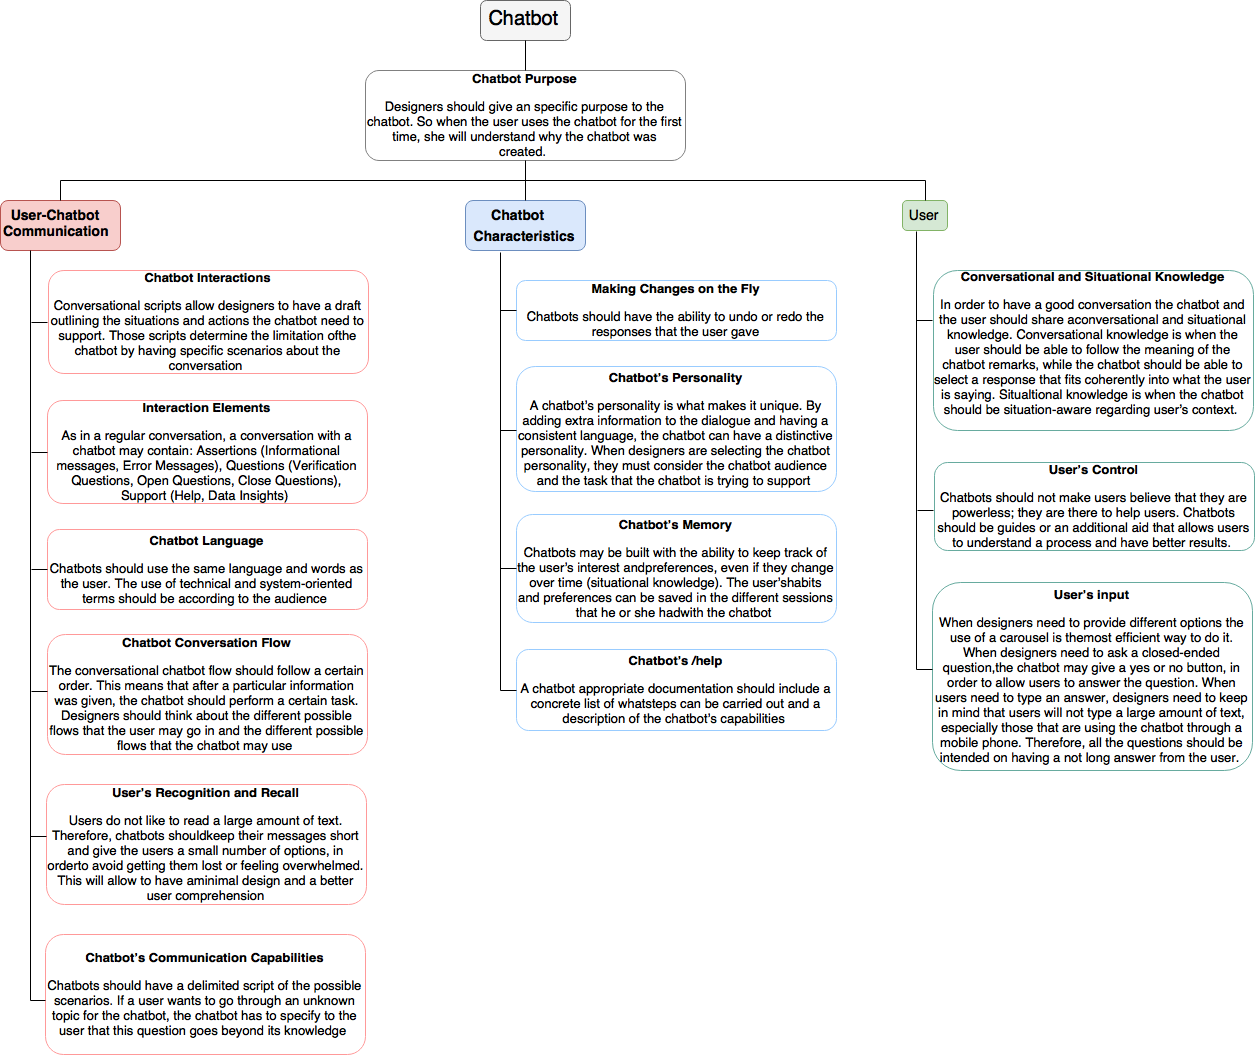
\includegraphics[width=1.6\linewidth]{/Users/MariaFerman/Desktop/ToRead(Project:Bots)/imgDesignfesst/BestPracticesDiagram.png}
    }
    \caption{Best Practices Diagram}
    \label{FigureBestPracticeDiagram}
\end{figure}

\textbf{Chatbot:} The goal of the chatbot is to help people like Laura to create a meaningful visualization about their data. Laura can use natural language statements in order to communicate with the chatbot. In response, the chatbot will provide her with several visualization options.

%Alexey's feedback: (on Visualizations: to communicate or to explore the data) 
\textbf{Chatbot's Tasks on Visualization:} The Visualization goal of the chatbot is to help users to analyse data by using visual context images (graphs). The chatbot will offer different options to visualize data. The options will be oriented to allow users to see patterns, trends, and correlations that might not be detected by the use of data tables or Excel sheets. Therefore, the chatbot will allow users to easily analyse their data in order to have deeper insights.  

The creation of a Visualization chatbot allows us to test the best practices of this project's first phase. A visualization chatbot was selected because Visualization is an emerging area that "allows people to analyse data when they don't know exactly what questions they need to ask in advance"\cite{munzner2014visualization}. Therefore, Visualizations help people in their decision making process by giving them evidence about the most important insights of their data.

Bringing chatbots into the visualization world allows users to get help to explore and analyse data, making the visualization creation process easier and more straightforward.  One example of Chatbots used to help people to visualize data is Iris~\cite{Iris}. Iris is a data science chatbot that allow users to get help with data science workflows (e.g. get a Person Correlation from a dataset). Another special task for Iris is its ability to create simple graphs from the user data (e.g. scatter plots, bar charts).    




%\newpage
%\null\vskip 2em\begin{Chatbot's Best Practices}
\begin{center}
	\section*{ Chatbot's Best Practices}
\end{center}

The following section describes 16 best practices to create a chatbot. The Chatbot's best practices and its definitions is being represented in Figure 4. The chatbot purpose is one of the most important best practices of this list. Based on the chatbot's purpose, designers can define the following chatbot's best practices sections: User-Chatbot communication, Chatbot features, and Human factor concerns. 

The \textbf{User-Chatbot communication} section represents all the interaction elements that users may have with a chatbot when they are exchanging information or ideas. The second section, \textbf{Chatbot features}, represents the characteristics that a chatbot may have. The final section, \textbf{Human factor concerns}, represents what factors are considered important by users when they interact with a chatbot.  

\section{Chatbot Purpose}

The purpose of a chatbot should be clear to its users. A chatbot that makes a user feel confused about its purpose is futile. \textbf{Designers should give a single purpose to the chatbot~\cite{ChatbotWord}. Users need to have a clear understanding of why the chatbot was designed and what its capabilities and limitations are.}

Currently, chatbots' designers can deal with this issue in two different ways. The first is to have a clear explanation about the chatbot's capabilities at the beginning of the interaction with the users. A clear example of a chatbot purpose definition is the CNN chatbot (cf. Fig. \ref{FigurePurpose}). When the user opens the chatbot for the first time, the chatbot describes the top stories and gives an explanation about how to get more news according to his or her preferences. The second option is to allow users to discover by themselves the purpose and capabilities of the chatbot during the interaction.

Chatbot designers need to identify a balance between the constraints of the interface and the user goals. Besides this, the kind of chatbot needed should be decided based on the final user requirements, and if it is feasible to create them or not. After finding this balance and making this analysis, the designers should define what the chatbot's capabilities will be (i.e., what the chatbot can do in order to help users in their tasks). 

In addition, designers should understand when to use a direct manipulation interface (e.g., graphic user interface) and when to use a chatbot. Usually, conversational agents that do not have a clear purpose make the user feel that the job can be done by a regular website. Chatbots can be very useful as long as they are well-developed and oriented to the purpose.  

 %According with Maes \cite{shneiderman1997direct}, if a designer wants to create an agent that will work and has the trust of the user, it is important to understand  

\begin{figure}
\centering
\includegraphics[scale=0.4]{/Users/MariaFerman/Desktop/ToRead(Project:Bots)/LaTexImages/CNN_chatbot_purpose.png}
\caption{CNN Chatbot}
\label{FigurePurpose}
\end{figure}

% I
\section*{I User-Chatbot Communication}

This section represents the elements that a session with a user and the chatbot may have when they are exchanging information or ideas.  

\section{Chatbot Interactions Scenarios}
Interaction is defined as the action or influence of things on one another \cite{merriam-webster}.
%According to the Cambridge dictionary, interaction is defined as the occasion when two or more people or things communicate with or react to each other!!!!!.
Chatbots should have a well-designed series of interactions with their users. Every single intended interaction should have a specific script of the different conversations that the chatbot and the users may have. 

\textbf{\textit{Conversational scripts}} \textbf{allow users to have a ``draft outlining the situation and actions the chatbot needs to support"~\cite{CaseStudy}. Those scripts determine the limitation of the chatbot by capturing specific scenarios about the conversation.} 

%moved-from conversation flow
Chatbots need to follow a conversational script that is a structured development of the conversation \cite{SmartNotesforBuildingaFeaturedBot} to avoid references that are not clear to the participants and engage users in the conversation.

%moved-from conversation flow
The conversation between the user and the chatbot should not lead to any ambiguity. Therefore, the chatbot's conversation should be structured and have messages that are clear and concise. By using a structured conversation, chatbots can guide a user through the interactions~\cite{HeuristicsWebPage}.


One of the most important and complex parts of designing a chatbot is the creation of the conversational script, because the user can take many paths (i.e., conversation scenarios) in order to achieve one task~\cite{designChatbotConversatio}. In other words, users can follow different paths which should all arrive at the same destination. One effective way to create those different scenarios is using mind maps. According to Eppler~\cite{eppler2006comparison}, ``Mind maps are defined as a a multicoloured and image centred, radial diagram that represents semantic or other connections between portions of learned material hierarchically." Figure \ref{FigureMindMap} shows a mind map regarding the different conversational scenarios of a chatbot that allow novice users to create visualizations. 

%\begin{figure}
%\includegraphics[scale=0.23]{/Users/MariaFerman/Desktop/ToRead(Project:Bots)/imgDesignfesst/ConversationalMindMap.png}
%\caption{Visualization Chatbot's Conversational Mind Map}
%\label{FigureMindMap}
%\end{figure}

\begin{figure}
    \makebox[\linewidth]{
        \includegraphics[width=1.7\linewidth]{/Users/MariaFerman/Desktop/ToRead(Project:Bots)/imgDesignfesst/ConversationalMindMap.png}
    }
    \caption{Visualization Chatbot's Conversational Mind Map}
   \label{FigureMindMap}
\end{figure}

After creating the mind maps, designers may use tools like InVision\footnote{www.invisionapp.com} in order to create the conversational chatbot mockups.

As in a human conversation, chatbots and users can have the same parts of a conversation such as greetings,  conversation and farewell. The following subsections give a further definition of those conversational parts.

\subsection{Greeting}
From the first interaction between a user and a chatbot, the user should have a clear idea of the chatbot purpose and what he or she can expect from it. Therefore, the user should know the context in which the chatbot needs to be used.

The welcome or greeting section is the first interaction in which chatbots should clearly communicate their purpose, in order to avoid functionality misunderstandings (cf. Fig. \ref{FigurePurpose}). 
%According to Lurchenko, the information in the welcome screen should not exceed 160 characters~\cite{CheatSheet}. 
The welcome section of the conversation should be short and concise, to avoid users feeling overwhelmed due to the amount of information provided by the chatbot. The first section of Figure \ref{FigureMindMap} shows the \textit{greeting conversational script} for a Visualization chatbot. This section shows the possibles greetings that a user may utilize for starting the conversation with the chatbot.  

\subsection{Conversation}
The conversation section is when the topic will be developed. According to Mishra ~\cite{effectivCommunication}, ``Effective communication is getting the message across as intended and getting desired feedback by influencing and attracting attention". The chatbot's conversation ``should provide information the user wants to know"~\cite{HowChatbotsCanHelpUsers}. Therefore, chatbots should be able to express a clear message to the user in order to have an effective communication. This section can have assertions, questions, comments, and feedback. The participants of the conversation should take turns interacting in order to communicate a clear message. A conversation with a visualization chatbot may have the following sections: \textit{Visualizations, More visualizations, Help, Refactoring, Undo, and Non-supported expressions} (cf. Fig. \ref{FigureMindMap}).

\subsection{Farewell}
The farewell section is the last part of a conversation. By this phase, the user should have had the help that they needed in order to finish their task and to have relevant feedback. In this section, the chatbot should ask the user if the provided information or help was useful, and if the user would like to do anything else. The last section of Figure \ref{FigureMindMap} shows the \textit{farewell conversational script} for a Visualization chatbot. 
%------------------------------------------------------------------------------------------------------------------------------------------------------

\section{Chatbot Interaction Elements}
According to Allen et al.~\cite{allen1978conversation}, Interaction can be defined as the "reciprocal process incorporating a variety of verbal and somatic components which are organized into meaningful action segments transmitted from one actor to the other in an oscillatory pattern." The authors claim that \textbf{the speaker can emit several elements, such as assertions, questions, and support in a conversation.} The interaction elements can be emitted by humans and chatbots when they are interacting with each other. The following interaction elements are described from the chatbot's perspective. 

%https://www.socialresearchmethods.net/kb/questype.php

\subsection{Assertions}
Assertions are affirmations or messages that the chatbot gives to the user; assertions determine the content of the conversation and allow the listener to increase his or her knowledge about a certain topic. 

\subsection{Questions}
Questions can be used to make sure that the provided information is required by the user. Stivers \cite{stivers2010overview} classify questions according to the expected answer and according to the question's goal. Below are described the two question's classifications. 

\subsubsection{Questions based on the response}

According to Stiver et al,\cite{stivers2010overview} Questions should be designed by the type of answer the speaker wants to get. For example, if the speaker what to have a yes or no response, a clausal answer or the choose between two options.
\begin{enumerate}
\item Polar or close-ended questions: Polar questions are formulated to get the confirmation or disconfirmation of a topic. Thus, this kind of questions is answered with only two options, yes or no (True or false). Polar questions are subdivided in interrogative, Tag and Declarative. 
\begin{itemize}
\item Interrogative: Interrogative questions are stuttered as follows: the operator then the subject, this kind of questions are pronounced by a rising intonation.
\item Tag: Tag questions has a bigger extend function than other types of questions. \cite{quirk2010comprehensive}. This type of questions is not that common in the English language. Some examples are \textit{isn’t she?, did she?, right?, huh?} 
\item Declarative: Declarative questions are pronounced with a casual tone in spontaneous or casual conversations.
\end{itemize}
An example of a polar question is when Poncho\footnote{https://poncho.is/}, the weather forecasts chatbot, asks users about the city for which they want to know the weather. If the user would like to know the weather in Manhattan, Poncho will ask the following verification question, ``New York, NY? Right now it's mostly cloudy there. Is that the right city?" and after the user clicks "yes" Poncho will give the complete forecast (cf. Fig. \ref{FigureVerificationQuestion}). 
\item Q-word (or content questions): Q-word questions are asked when a “part of a proposition is presupposed, and the utterance seeks the identity of one element of the proposition”\cite{stivers2010coding}. This type of questions use the following words: \textit{who, what (adjective values), where (location), when (time), why (cause) and how (manner)}. In some conversations, Q-word questions may be preceded by the words and, but or so. For example “So why didn’t Laura eat with him? 
\item Alternative: Alternative questions are occasionally used in English conversations. This type of questions joins two complete questions by using the word \textit{or}. Therefore, the answer to this type of questions is the election between two restricted set of alternatives. For instance, You would like to eat flour tortillas or you prefer to eat corn tortillas?
\end{enumerate}

\subsubsection{Questions based on the objective goal}
Stivers also gives a classification of the social action (objective/goal) that the questions are intended.  
\begin{enumerate}
\item Request of information: Questions are formulated to request information when they are asked in order to get information and no other primary action is implied in the question. In other words, questions like “Are you busy tonight” hide another primary action that may be an invitation request. 
\ item Other initiation of repair: Tag questions are formulated to other initiation of repair. The objective is to get a partial repeat. For example,  isn’t she?
\item Request for confirmation: Declarative questions may be formulated to confirm some information. For instance, ‘So you’re coming tomorrow night’’. 
A chatbot may ask to confirm its correctness before carried out a process. \cite{Shevat2017}
According to Shevat \cite{Shevat2017}, there are two types of confirmation that bots may use, explicit and implicit. Explicit is when the chatbot asks for the correctness about an input provided by the user. They are also used to allow the chatbot to ask the user permission to carried out a task (process).  On the other hand, implicit confirmation is when the chatbot confirms to the user that it receives the user’s input. 
\item Assessment: this social action is carried out to seek an agreement, an example of this is “Isn’t it beautiful out today" 	
\item Suggestion/Offer/Request: This category of questions are formulated to suggest, propose and offer something to a person. They also included questions that are being asked to request something. For example “Do you want some chocolate cake?” 
\item Rhetorical question: This question does not seek for an answer. They are being created to express an opinion. For example, ‘‘Everything comes out in the wash doesn’t it? said by a husband to his wife after he has spilled something on the table cloth” \cite{stivers2010coding}.
\item Outloud: Outloud questions are not formulated for someone in particular, they just express a thought outloud. (e.g., “Now where did I park the car”.
\end{enumerate}

Another type of questions is open-ended questions. This type of questions allows individuals to spontaneously give an answer, avoiding the bias of giving them alternatives that may influence their response \cite{reja2003open} . 

%Open and close questions: https://robinhq.com/customer-service-guide/human-conversation/

\begin{figure}
\centering
\includegraphics[scale=0.3]{/Users/MariaFerman/Desktop/ToRead(Project:Bots)/imgDesignfesst/VerificationQuestion.png}
\caption{Poncho Weather Forecast Chatbot: Example of an Close-ended question}
\label{FigureVerificationQuestion}
\end{figure}

However, designers should avoid open-ended questions, because users may respond in a non-supported way. A solution for this may be the use of questions that provide different options in buttons inside the chatbot message as shown in figure \ref{FigureVerificationQuestion}, and the chatbot should ask users to select one~\cite{ConversationalUXDesignFacebook}. Each provided option will invoke different actions. If the options provided by the chatbot contain several images, a good way to display them is the use of carousels~\cite{carousel} (see best practice User's input).

%to be include?
%To add Persistent menus - menus that are in teh interface not in the bot. always available information.  
% https://chatbotsmagazine.com/cheat-sheet-all-facebook-chatbot-interactions-4b14e4e00178

\subsection{Support}
Finally, support is any extra help that the chatbot gives to the user. Support can be divided in three categories, help, feedback and data insights.
\begin{enumerate}
\item Help: the help provided by the chatbot should be straightforward for users, it should give a possible solution when the user get stuck in the conversation. Chatbots should have a specific script about how to use the chatbot. Commonly, users only need to type the word ``\textit{help}" or the command ``\textit{/help}" in order to get additional support from the chatbot. When an error has occurred the chatbot should automatically ask users if they need any help. 

\item Feedback: Chatbots can also give feedback as a part of the conversational support, or provide meaningful insights about the performed task or the conversation that the user and the chatbot had. According to Allen et al [26] Feedback may go from the receiver to the emitters, in this case, the receiver emits cue responses that allow the emitter to incorporate the feedback into the monitoring process. The feedback may also go from the emitter to the receiver, in this case, the verbal cues came as a response to cue responses from the emitter. 
Besides, chatbots may ask for a feedback from users in order to get an idea of the chatbot performance. Questions like “the provided information was useful” may give an idea to designers of the level of user’s satisfaction. 

\item Data insights: Chatbots may be used to provide additional information about the data provided by the user. One example of this is Watson Virtual Agent \cite{SuzorCustomerAnalytics}. This chatbot allow business to have rich insights about the customers that are using the chatbot for customer service. Customers chat with Watson, while business gets the data insights about the main customers’ needs and how many customers are using the bot. 
\end{enumerate}


Besides regular human conversational elements, \textbf{chatbots may also understand command expressions.} These statements are commands that users write to interact with the chatbot using domain specific knowledge. 



%\section{Conversational Script}
%The conversational script should take into account the following elements: timing, being an active participant and an active listener, and avoiding over sharing information.

%The chatbot's messages elements can include text, emojis, attached files, images, video or audio. The message can be structured; these types of messages follow the command line format and usually have buttons to allow users to get information or to answer a question previously asked by the chatbot. The content of the message should be short in order to have a minimal design and a better user comprehension.  %According to Lurchenko the content of the buttons should not exceed 20 characters including spaces~\cite{CheatSheet}. Besides, the font of the message should be in an adequate size, besides it can have bold, italic, fixed-width text, and inline links. 
%------------------------------------------------------------------------------------------------------------------------------------------------------
\section{Chatbot Language}
According to Allen et al.~\cite{allen1978conversation}, in order to have a meaningful conversation, it is necessary to share a language and have vocabulary in common. \textbf{Chatbots should use the same language and words as the user. The use of technical and system-oriented terms should be according to the audience.} 

 If the design of the conversational agent is oriented to certain populations, chatbots can mimic how users normally speak.  Therefore, before the creation of the chatbot, it is necessary to have a ``solid understanding of the audience we seek to appeal to, and to have a vocabulary familiar to them”~\cite{HeuristicsWebPage}. Figure \ref{FigureIRIS} shows a conversation between a user and Iris\footnote{https://github.com/Ejhfast/iris-agent/}, the data science chatbot. Iris is oriented to a scientific audience, therefore the language, that Iris uses, is according to a domain specific area.  

\begin{figure}
\centering
\includegraphics[scale=0.4]{/Users/MariaFerman/Desktop/ToRead(Project:Bots)/imgDesignfesst/IRIS-image.png}
\caption{Iris Data Science Chatbot}
\label{FigureIRIS}
\end{figure}
%------------------------------------------------------------------------------------------------------------------------------------------------------
\section{Chatbot Conversation Flows}
According to Reichman~\cite{reichman1985getting}, in a usual conversation many details are being shared. To avoid an incoherent conversational flow, it is necessary that individuals understand when and why the conversational topic has been changed. \textbf{The conversational chatbot flow should follow a certain order. This means that after a particular information is given, the chatbot should perform certain task.} 

\textbf{Designers should think about the different possible flows that the user may follow and the different possible flows that both the chatbot and the individual may use.} Users and chatbots can change the topic of the conversation at any point. Shifting the conversation topic should be made carefully to avoid misunderstandings. For example, eBay's ShopBot\footnote{https://shopbot.ebay.com/} helps users selecting a pair of jeans, and after that, the user can also ask for a blouse from a different department (cf. Fig. \ref{FigureEbay}). It is important to understand that the purpose of the conversation did not change, the purpose remains the same, that is buying clothes. However, the flow of the conversation switches from buying jeans to blouses from a different department.
%Another example is Poncho, users can ask him about the weather, and then change the conversation's topic and have a little chat with Poncho about astrology. 
\begin{figure}
\centering
\includegraphics[scale=0.4]{/Users/MariaFerman/Desktop/ToRead(Project:Bots)/imgDesignfesst/ShopBot.png}
\caption{ShopBot Ebay}
\label{FigureEbay}
\end{figure}
%* For instance, the design of the chatbots can twist the conversation from talking about a certain graph and when the user has selected the graph, to what color is better to use /find another example/. Shifting the conversation topic should be made carefully to avoid misunderstandings.  * 
Chatbots may change the flow of a conversation according to the chatbot purpose, an example of this is Rescue.io (cf. Fig. \ref{FigureRescue}). This chatbot was created to aim emergency situations. According to Clegg "during an emergency when the user cannot phone someone for help, Rescue can quickly alert the user's emergency contacts to what is happening and where the user is so they can help"~\cite{Rescue}. Rescue leads the conversational flow by asking a series of questions about the type of emergency that the user has. 
\begin{figure}
\centering
\includegraphics[scale=0.5]{/Users/MariaFerman/Desktop/ToRead(Project:Bots)/imgDesignfesst/rescued.png}
\caption{Rescue.io Emergency Chat Service}
\label{FigureRescue}
\end{figure}
%after 2 script parrafos
%However, designers should be careful of not letting the chatbot lose the feeling of a normal conversation. Some conversations might be structured too rigidly; for this reason they seem to be a command line, instead of giving the user the conversational feeling that chatbots should have. The flow of the conversation should be natural and evident. 
%------------------------------------------------------------------------------------------------------------------------------------------------------

\section{Chatbot's Communication Limitations}

\textbf{Chatbots should have a delimited script of the possible scenarios (cf. Fig. \ref{FigureMindMap}). If a user wants to go through an unknown topic for the chatbot, it is expected to notify the user that this question goes beyond its knowledge. Therefore, designers need to not only consider what the chatbot can do, but also what it cannot do, in order to set boundaries.} For example, when a user asks Poncho, the weather chatbot, something that it was not created to answer, Poncho replies with: ``Oops, I didn't catch that. For things I can help you with, type \textit{help}"~\cite{HeuristicsWebPage} (cf. Fig. \ref{FigureCommunicationCapabilities}). Chatbots need to gracefully establish limits to users that go beyond the chatbot's knowledge.  

\begin{figure}
\centering
\includegraphics[scale=0.5]{/Users/MariaFerman/Desktop/ToRead(Project:Bots)/imgDesignfesst/PonchoHelp.png}
\caption{Poncho Weather Forecast Chatbot}
\label{FigureCommunicationCapabilities}
\end{figure}
%------------------------------------------------------------------------------------------------------------------------------------------------------

% II
\section*{II Chatbot Features}

\section{Chatbot's Personality}

Personality is defined as the combination of characteristics or qualities that form an individual's distinctive character~\cite{Oxford}. \textbf{A chatbot’s personality is what makes a chatbot unique. By adding extra information to the dialogue and having a matching language, the chatbot can have a distinctive personality.} However, designers should be careful to not include too much additional information that makes the user feel bored or annoyed. There has to be a balance between giving just the relevant information and adding extra information to make the chatbot's conversation more engaging. Moreover, the chatbot personality is an important part to make the user more engaged with the interface.

The chatbot’s personality should take into account the target audience for which it was designed. The personality should match with the users, therefore, how friendly, sarcastic or humorous should only depend on the people who will use the chatbot. \textbf{It is very important that the design of the personality considers the chatbot audience and the purpose that the chatbot is trying to support.}  

Users like to interact with chatbots in a human way~\cite{HeuristicsWebPage}. For this reason designers should consider how to engage users in the conversation. 

A clear example of how to get user engagement is the Aura's Bot\footnote{http://m.me/aurapower}. Aura Dione is a Danish singer who is using a chatbot in order to be in contact with her fans. The designer of the Aura's Bot uses the personality of the singer. (cf. Fig. \ref{FigureAura}). Therefore, the tone of the chatbot is like an artist, and fans can communicate with it and ask extra information about the singer. Fans have the feeling of interacting with the singer, and this leads to the user engagement and retention~\cite{personality}.  

\begin{figure}
\centering
\includegraphics[scale=0.4]{/Users/MariaFerman/Desktop/ToRead(Project:Bots)/imgDesignfesst/AuraBot.png}
\caption{Aura's Bot}
\label{FigureAura}
\end{figure}

According to Scott~\cite{HeuristicsWebPage}, there is a difference between the content (\textit{relevant information to help the user}) and the medium (\textit{the chatbot’s personality}). Users need to be entertained and at the same time to be helped.      

%Spectrm establishes a series of questions in order to select the right personality for a chatbot: ``Do you have a mascot (for a product or brand)? Does this mascot have a personality that might serve as inspiration? Is there a core value for your company in general or to its way of communication that could inspire the personality? Can you think of a person you know, a celebrity or a fictional character that your bot could resemble?" \cite{personality}. Those questions allow designers to create a template or structure about how they want the chatbot to behave and interact with the users.

Other important considerations to take into account are the age, heritage, friends and occupation that the chatbot may have. All these specifications enable designers to have a clear definition of whom the chatbot will resemble.

To summarize, the chatbot’s success may be defined by how designers balance between entertainment and guidance. Therefore, the difference between chatbots that are being used and those that are not, is how compelling and pleasant the chatbot experience is.

%\section{Chatbot's Audience - Should be a subsection of Personality?}

%Chatbots can be developed for business, customer oriented tasks, or just be oriented to teen customers~\cite{Shevat2017}. Business oriented tasks' chatbots are designed to help teams to collaborate in a more effective way. This kind of chatbots can be useful to help software developers in their task because ``it can help reduce the friction points they have to face when working collaboratively"~\cite{lebeuf2017software}. An example of a business oriented task chatbot is the slackbot\footnote{https://api.slack.com}. The consumer oriented tasks' chatbots are designed to help users communicate, get additional information or help. An example is Poncho the weather forecast chatbot. Finally, the teen oriented chatbots are developed to entertain young customers and these kinds of users like to play games, chat and share content with friends. An example of this chatbot is Kik\footnote{https://bots.kik.com/}. 

%According to Shevat, in order to define the chatbot's audience, developers need to answer the following questions: Are you addressing a business use case? Is this a consumer use case? Are you targeting teens? Families? Adults at work? When are they using the service? \cite{Shevat2017}.

%\section{Chatbot's Versatility}
%retrival base bots - question answer 
%Chatbots should be versatile enough to be able to understand open-questions, commands, and requests written by the user. An example of an open-question is when users ask Poncho, "What's the weather like in Brooklyn this weekend?" and then Poncho answers with the Brooklyn weather forecast. 

%However, if a user wants to use a command in the interaction with the chatbot, the dialogue should continue smoothly without breaking the flow. Commands to chatbots can be conveyed via special characters followed by an argument. For example, chatbots' commands in Slack and Telegram start with a slash follow by an argument. The characters of the argument can be Latin letters, numbers and underscores~\cite{botfather}. It is a common practice to have slash commands in the following pattern: slash ``command name" ``arguments"~\cite{Shevat2017}.  
%------------------------------------------------------------------------------------------------------------------------------------------------------
\section{Chatbot's Memory}

\textbf{Chatbots should be built with the ability to keep track of the user's interest and preferences, even if they change over time \textit{(situational knowledge)}. Conversational agents can save the user's habits and preferences in the different sessions that he or she had with the chatbot}~\cite{shneiderman1997direct}. As an example of this, Poncho can save the location of a certain user. Therefore, the next time that the user asks for a weather broadcast, Poncho already knows which location to look at, saving the user time and keystrokes. Besides, these allow the user to have a customised experience. 

%If I come back, Poncho will remember my location, saving me a few keystrokes.*
%------------------------------------------------------------------------------------------------------------------------------------------------------
\section{Making Changes on the Fly}

It is normal that users make mistakes when they are choosing different options in an interface. \textbf{It is very important that chatbots have the ability to undo or redo users responses.} In that case, users know that they are able to undo an unwanted change triggered by a misinterpreted message or a mistaken click~\cite{HeuristicsWebPage}. %Therefore, designers must take into account that users may make mistakes. 
Figure \ref{FigureUndo} shows an example of a chatbot without the undo capability. In this example, the user made a mistake in the items added to the shopping cart. Because the chatbot does not have this ability, the user has two options, start the conversation from the beginning or buy all the items that are in the shopping cart even if he or she does not need them. This is a good example of why chatbots need to provide this functionality, because users will feel annoyed of starting the whole conversation again or may not be willing to purchase mistaken added items. 

During a conversation, Chatbots have hints about when a user made a mistake. In the previous example, when the user said ``I meant" is a clear indication of the user made a mistake. Therefore words as ``meant" gives designers a clue of when to use the undo capability.

Another approach is that the chatbot directly asks users if the information provided is accurate. The Poncho chatbot has the ability to ask users if the information provided was appropriate; if not, users can clarify it.  

\begin{figure}
\centering
\includegraphics[scale=0.5]{/Users/MariaFerman/Desktop/ToRead(Project:Bots)/imgDesignfesst/Undo2.png}
\caption{Chatbot Without an Undo Capability}
\label{FigureUndo}
\end{figure}

%\section{Error Messages}

Chatbots should express error messages in a straightforward way. According to Armstrong~\cite{HelpingYourBabyBotLearnToChat}, Chatbots should be able to express that they did not understand and re-ask to the user to repeat their message in a different way. If necessary the chatbot should give different answers when it did not understand the user, in order to avoid the user deal with the same message over and over again. After several error messages in a row, the chatbot should give a report a problem or send feedback option. 

%Error prevention allows users to understand that something unexpected just happened in the interaction. For example, an error can be a wrong input data from the user. In the case of such an event, the chatbot should allow users to get additional help or undo what they have just done. Some chatbots  allow to speak with a live agent in the event that the user is struggling with the chatbot interaction. An example of this is 1-800-Flowers Assistant~\footnote{https://www.facebook.com/1800FlowersAssistant/}, this conversational agent can connect a live agent if the conversation with the chatbot fallows for a certain period of time. 

%To summarize, a good chatbot should be able to provide evidence around error prevention and allow users to recover when an error just happened~\cite{HeuristicsWebPage}. 
%------------------------------------------------------------------------------------------------------------------------------------------------------
\section{Social and Emotional Intelligence}

Another significant challenge that designers need to keep in mind is \textbf{giving the chatbot social and emotional intelligence. Therefore, the chatbot should be sensitive to users preferences.} According to Siegel et al.,~\cite{siegel2012pocket}, ``Social and emotional intelligence can be defined as skills that enable an individual to understand the impact of emotions on behavior and thinking, to regulate emotions and behavior, to understand the importance of emotions in others, and to understand social interactions and engage in adaptive ways with others in social situations."

\textbf{Chatbots should be helpful without being annoying}. A good example of this is the Microsoft Office Assistant ``Clippy the Paperclip” (cf. Fig. \ref{FigureClippy}). Some of the most well-known of Clippy's problems were the random interruptions to users asking them if they need help writing a letter, movement and winking at odd intervals, distracting users \cite{Clippy2015}. According to Shneiderman~\cite{shneiderman1995looking} ``The anthropomorphic styles are cute the first time, silly the second time, and an annoying distraction the third time.”

\begin{figure}
\centering
\includegraphics[scale=0.7]{/Users/MariaFerman/Desktop/ToRead(Project:Bots)/imgDesignfesst/Clippy.png}
\caption{Microsoft Office Assistant Clippy the Paperclip}
\label{FigureClippy}
\end{figure}

\textbf{Chatbots help users by ``chatting" with them and being guides for a certain task that the user needs to perform. Therefore, chatbots that have the ability to save user preference should be careful enough to not share personal information with other users}. An example of this is Xiaoice, a chatbot developed by Microsoft. Xiaoice is an artificially intelligent software program designed to chat with people. This chatbot can be used in group conversations, and there is evidence that Xiaoice has revealed (in the group conversation) personal information gathered from one-to-one sessions~\cite{TheChallengeOfDesigningAChatbotWithManners}.     

In summary, designers should keep in mind that the chatbot should help users in an appropriate time and give relevant information to help them. Besides, chatbot's designers should always keep in mind what the users' preferences are. 


   
%https://www.accenture.com/t20161212T073257__w__/nl-en/_acnmedia/PDF-1/Accenture-Strategy-Workforce-IQ-EQ.pdf
%partnering with people to radically improve the emotional intelligence and social relationships of the workforce of the future

%https://chatbotsmagazine.com/helping-your-baby-bot-learn-to-chat-like-a-grown-up-bot-99f5170f1c55
%scenarios
%https://chatbotsmagazine.com/how-chatbots-can-help-your-users-without-you-there-e82e6814a903

%https://conferences.oreilly.com/design/ux-interaction-iot-us/public/schedule/detail/54917?intcmp=il-design-confreg-lp-dsca17_20161214_new_site_five_questions_desiree_garcia_session_text_body_link

%https://www.fastcodesign.com/3064710/the-challenge-of-designing-a-chatbot-with-manners

%------------------------------------------------------------------------------------------------------------------------------------------------------
\section{Chatbot's /help}

Chatbots should be used without the need for extra information. How to use a chatbot should be a simple conversational flow. However, there are some users that like to deeply understand how the interface works and detect its limitations. \textbf{A chatbot appropriate documentation should be precise and short. It should provide extra information about how the chatbot can help users in their tasks.} Besides, it also should include a concrete list of what steps can be carried out and the critical points of the chatbot~\cite{HeuristicsWebPage}. 

Finally, the chatbot should provide an easy way to access the documentation. One example of this is when the user types slash ``/" and a list of the supported commands of the chatbot should appear on the screen~\cite{botfather}.  
%------------------------------------------------------------------------------------------------------------------------------------------------------

% III
\section*{III Human Factor Concerns}

\section{Conversational and Situational Knowledge}

Conversations need to follow certain rules and to have a certain semantic order for the sake of having a clear understanding between the user and the chatbot. Therefore, in order to have a good conversation the chatbot and the user should share a conversational and situational knowledge. 

%The chatbot script should follow the same rules and semantic order as a regular conversation. In other words, there should be a mapping between the script and the actual conversation. Designers need to understand what the actual conversation will feel like for the users and then create the chatbot accordingly. 

\textbf{\textit{Conversational Knowledge}} \textbf{is when the user is able to follow the meaning of the chatbot's remarks, while the chatbot is able to select a response that fits coherently into what the user is saying.} Therefore, it is vital to understand how chatbots and users follow each others' thoughts. In other words, Conversational Knowledge is the common definitions in the conversation that do not change over time. 

Figure \ref{FigurePoncho} shows the user asking Poncho to have the temperature in Celsius rather than Fahrenheit degrees. In this example, the temperature units are the shared conversational knowledge. For this reason the user request makes sense in the conversational context, and the chatbot is able to make the conversion of the temperature.     


\textbf{\textit{Situational Knowledge}} is another important part of having a mutual understanding in a conversation. According to Reichman~\cite{reichman1985getting} people need to share Situational Knowledge in order to understand and follow a conversation because it involves previous knowledge about the topic that is being discussed.  

In a user-chatbot conversation, Situational Knowledge \textbf{is when the chatbot is situation-aware regarding the user context.} Therefore, Situational Knowledge change over time according to the user's context. Figure \ref{FigurePoncho} shows a user asking ``What is the temperature in London right now?" Due to Poncho and the user share the same situational knowledge about the current time, the provided forecast will be according to the time, when the user asked the information. 

%Listeners must be able to follow the context of the conversation; they need to grasp what the speaker's point is and what he or she said before. Listeners need to understand the prior and the current context of the conversation to avoid being confused and to grasp the conversation's assertion. At the same time, speakers need to follow the order of a conversation to make their remarks easily understandable to the listeners. Therefore, the user and the chatbot should \textit{share the same information, to be on the same page.} 

\begin{figure}
\centering
\includegraphics[scale=0.2]{/Users/MariaFerman/Desktop/ToRead(Project:Bots)/imgDesignfesst/PonchoConversationLines.png}
\caption{Poncho Weather Forecast Chatbot}
\label{FigurePoncho}
\end{figure}
%------------------------------------------------------------------------------------------------------------------------------------------------------
\section{User's Control}

Users are accustomed to and like having control over the software. For instance, when a user has the ability of doing more customizations in an interface, they tend to feel more engaged in using that interface, because it has the user preferences. Therefore, it is extremely important to make the user feel that he or she has control over the interface. According to Maes~\cite{shneiderman1997direct}, ``users must be able to to turn over control of task to conversational agents but users must never feel out of control".

\textbf{Chatbots should not make users believe that they are powerless over the interface; they are there to help users to have a better experience using the interface. Chatbots should be guides or an additional aid that allows users to understand the interface and have better results.} According to Shneiderman~\cite{shneiderman1997direct}, it is ``necessary to give the users the feeling of being in control and therefore they can be responsible for the decisions they make.” 
%------------------------------------------------------------------------------------------------------------------------------------------------------
\section{User's input}

\textbf{There are several ways that the chatbot may receive the input from a user, by clicking an image in a carousel, clicking buttons or by directly typing a message in a text box, among others.} And designers need to have a clear understanding about when is a better option for users to click rather than type. 

When chatbots need to provide different options, from which the user need to select one, the use of a carousel is the most efficient way. According to Pernice~\cite{carousel}, ``Carousels enable more than one piece of content to occupy the same piece of prime real estate on the homepage, which can help diffuse any infighting about whose content is most deserving" and it should not be included more than five frames in each carousel because it is hard for users to remember more than five topics at the same time.

When chatbots need to ask a closed-ended question, the chatbot may give a yes or no button, in order to allow users to answer the question. 

When users need to type an open-ended answer, designers need to keep in mind that users will not type a large amount of text, especially those that are using the chatbot through a mobile phone. Therefore, all the questions should be intended on having a not long answer from the user. Besides, it is also difficult for the chatbot to understand the user's intent from a long paragraph. 

 
%------------------------------------------------------------------------------------------------------------------------------------------------------
\section{User's Recognition and Recall}

According to Scott, \textbf{users do not like to read a large amount of text: ``they will read the first message and then their eyes glaze over. They skim the rest of the text”}~\cite{HeuristicsWebPage}. The principle of least effort, set forth by Zipf, also specifies that people use shortened words and expression in speech, in order to obtain the maximum communication by using the least cost~\cite{zipf2016human}. \textbf{Therefore, chatbots should keep their messages short and give the users a small number of options, in order to avoid users getting lost or feeling overwhelmed. This will allow to have a minimal design and a better user comprehension.}

In addition, users do not remember details of the options given by an interface. When users avoid reading a large amount of text, they may misunderstand the chatbot’s message and finish with an unsuccessful result. The design of the chatbot dialogue should only have relevant information to help users with their tasks and prevent a dull interaction with the chatbot. 
%... p.8
%------------------------------------------------------------------------------------------------------------------------------------------------------
\section{Ethics- Data Security and Privacy (still deciding the title)}
We have reached to a point in which we should beware of what type of information we are sharing with an interface. We have the same issue with chatbots; users need to be careful about what data to share with a chatbot. \textbf{Chatbots' designers must have a \textit{code of conduct} for chatbots. Therefore, chatbots need to tell users ``which steps of data is processed in the background when talking to a bot"~\cite{PrivacyandDataSecurityofChatbots} and what measures that chatbots' designers took in order to protect users' privacy and data.} 

Users need to understand that when they are interacting with a chatbot is not a private and personal conversation between the user and the chatbot. Interactions are being recorded on servers, data is being saved into a database, and conversation records are being used to understand the user and save their preferences. According to Ondrisek~\cite{PrivacyandDataSecurityofChatbots}, ``All transactions are logged by the platform’s servers, which monitor and log the communication between the user and the bot, therefore bot's platform provider has complete access to the un-encrypted conversation."  However, some chatbots have dealt with these privacy concerns. According to Yao Baogang~\cite{ForSympatheticEar}, with Xiaoice (chatbot with the purpose to provide entertainment and companionship) ``We don’t keep track of user conversations with Xiaoice, we need to know the question, so we store it, but then we delete it. We don’t keep any of the data. We have a company policy to delete the user data."

%Therefore, when a user is interacting with a chatbot, he or she should be careful of what kind of information is being provided to the chatbot, because the conversation does not finish with the chatbot. 
Therefore, designers should treat users' data ethically, and inform if their information is being shared with third parties.   
%conclusion "Dependent on this data you receive you can create personality profiles of bot users. So be careful what you write with a bot and what data you expose on platforms."

%DATASET with visualization examples:
%2visualizations:
%https://www.empirecenter.org/publications/empire-states-half-century-exodus/

\section*{\centering{Mock-up of a Visualization Chatbot}}

%DATASET with 2 visualization examples:
%2visualizations:
%https://www.empirecenter.org/publications/empire-states-half-century-exodus/

%2visualizations:
%https://www.analyticbridge.datasciencecentral.com/profiles/blogs/same-dataset-two-different-kind-of-visualizations
%Dataset
%https://backhome.news21.com/interactive/suicide-interactive/

%Dataset & visualization explanations & R CODE!
%http://datajournalismhandbook.org/1.0/en/understanding_data_7.html

% 25 visualizations one dataset:
%https://flowingdata.com/2017/01/24/one-dataset-visualized-25-ways/
%https://www.wired.com/2017/02/25-visualizations-spin-data-25-different-tales/
%Dataset:
%http://apps.who.int/gho/data/node.country

%Tableu 3 vis (best but with dataset issue)
%https://www.tableau.com/about/blog/2016/2/one-data-set-multiple-views-introducing-reviz-project-50564
%Dataset
%https://www.cdc.gov/injury/wisqars/fatal.html

\section*{\centering{Case Study}}

	
\medskip

\bibliographystyle{unsrt}%Used BibTeX style is unsrt
\bibliography{References.bib}

\end{document}